Um das in Abschnitt \ref{subsec:dither sampling} vorgestellte \textit{Dither Sampling} zu realisieren
benutzen wir diese im Folgenden vorgestellten \glqq nachträglichen\grqq Annahmen. 
A Posteriori sind Sie in dem Sinne, als das wir die Annahmen szenenabhängig machen und Sie anhand 
von bereits erstellten Pixelwerten formulieren. Damit werden Sie unabhängig vom Integranden der Formel 
\ref{eq:concreteMonteCarlo}.

\subsection{Theoretische Grundlage}

Im Kapitel über den \nameref{ch:Content1:sec:Path Tracer} haben wir gesehen, dass 
wir den Wert eines Pixels (i,j) klassischerweise mit einem zufälligen
Startwert durch eine Monte-Carlo Integration erhalten. Wir betrachten im
Folgenden eine (theoretische) Menge aller möglichen Pixelwerte, welche durch alle möglichen Startwerte generiert wurde.
In Abbildung \ref{eq:Pixel Schätzung Wahrscheinlichkeitsdichtefunktion} ist die Wahrscheinlichkeitsdichtefunktion
$h_{ij}$, als eine Funktion über alle möglichen Werte $I_{ij}$ eines Pixels (i,j) aufgetragen.

\begin{equation}\label{eq:Pixel Schätzung Wahrscheinlichkeitsdichtefunktion}
    H_{ij}([I_{Anfang},I_{Ende}]) = \int_{I_{Anfang}}^{I_{Ende}} h_{ij} dI
\end{equation}

Verfolgt man beispielhaft die Werte eines Pixels über neun Bilder bei unseren \nameref{ch:Content1:sec:Path Tracer}, 
so ergibt es sich zur Anschauung wie folgt:

\begin{figure}[H]

    \begin{subfigure}{\textwidth}
        \centering 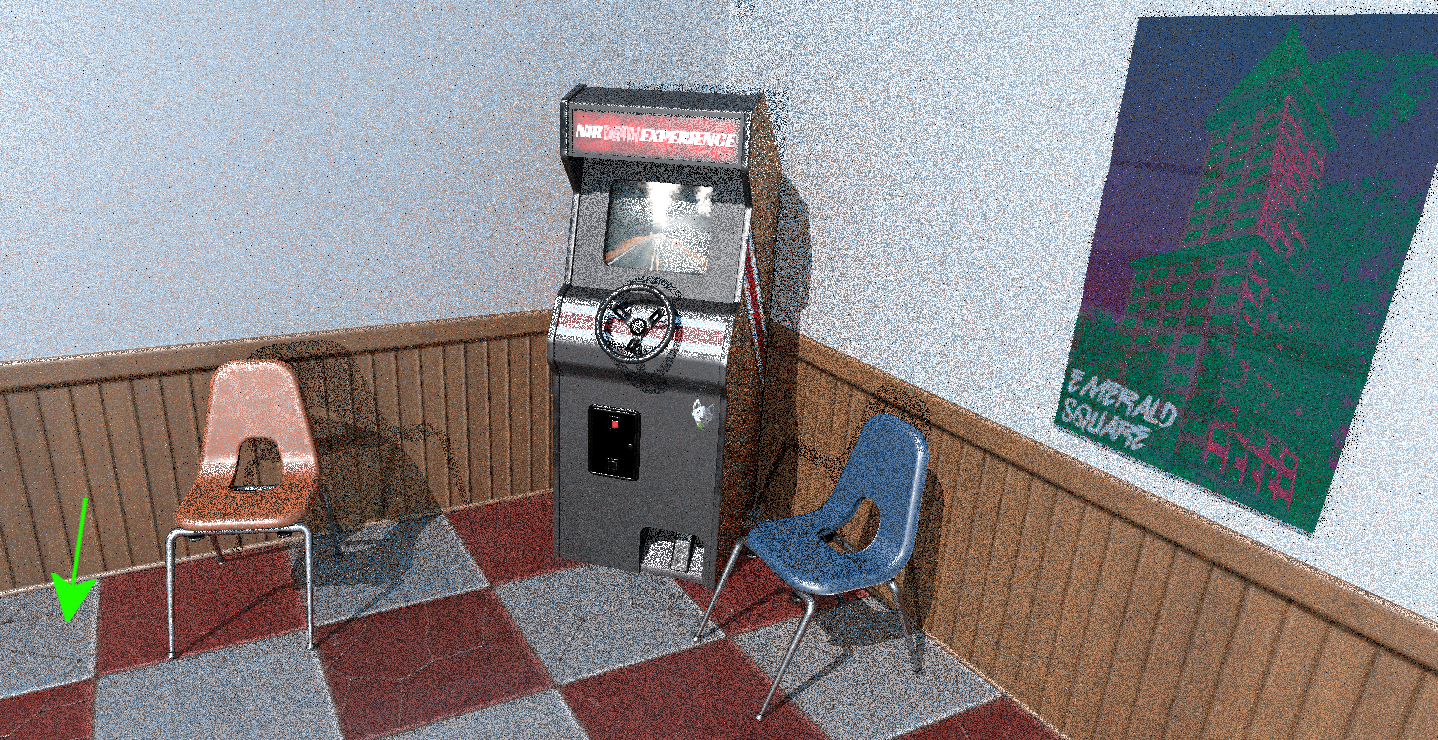
\includegraphics[width=0.5\linewidth]{content/TemporalerAlg/Bilder/APosteriori/Szenenausschnitt.png} 
        \caption{Szenenausschnitt}
        \label{fig:szene_pixel_position}
    \end{subfigure}

    \begin{subfigure}{0.5\textwidth}
        \begin{picture}(120,180)
            %\put(35,50){}
        \end{picture}
        \centering 
\includegraphics[width=0.6\linewidth]{content/TemporalerAlg/Bilder/APosteriori/pixel_512x512_strip.png} 
        \begin{picture}(120,30)
            %\put(35,50){}
        \end{picture}
        \caption{Werte des Pixels im zeitlichen Verlauf (grüner Pfeil)}
        \label{fig:ausschnitt_pixelstrip}
    \end{subfigure}
    \begin{subfigure}{0.5\textwidth}
            \centering
            \def\svgwidth{\columnwidth}
            \import{content/TemporalerAlg/Bilder/APosteriori/}{histogram_of_estimates.pdf_tex}
            \caption{Histogram der Pixelschätzungen}
            \label{pic:histogramOfEstimates}
    \end{subfigure}
        \caption{Pixelwerte (grüne Markierung) in aufeinanderfolgenden Zeitschritten}
        \label{fig:Pixelwerte}

\end{figure}

Betrachten wir im Folgenden allerdings die theoretische, zur Echtzeit nicht umsetzbare Menge aller möglichen Werte. 
Mit dieser Menge haben wir nun ein vollständiges Histogramm. Mit diesem Histogramm haben wir eine Wahrscheinlichkeitsfunktion 
der Pixelwerte $I_{ij}$ an Stelle (i,j). Dies bedeutet wiederrum, dass das Erzeugen eines 
Pixelwertes nichts anderes bedeutet, als eine zufällige Wahl anhand der impliziten
Wahrscheinlichkeitsdichtefunktion. Wir können folglich einem zufälligen Anfangswert einen konkreten 
Pixelwert zuteilen und eine umkehrbare Funktion definieren \ref{eq:inverse Funktion}. 

In Gleichung \ref{eq:inverse Funktion} lässt sich die Quantilfunktion $H_{ij}^{-1}(x)$ erkennen. 
Sie verdeutlicht die Zuordnung eines Anfangswertes zu einem konkreten daraus entstandenen Wert 
eines erzeugten Pixels.

\begin{equation}\label{eq:inverse Funktion}
    I_{ij} = H_{ij}^{-1}(x), x \in [0,1]
\end{equation}

\par

\textbf{Fazit}: Betrachte nun blue noise verteilte Zahlenfolge $d_{ij}$, die zum Erzeugen eines Pixelwertes herangezogen wird (wir erhalten eine solche 
Zahlenfolge für jeden Pixel mit gekachelter \nameref{ch:Content1:sec:blue noise}) Textur über das Bild). Unsere Quantilfunktion 
$H_{ij}^{-1}(x)$ ist monoton (da Sie die Inverse einer Wahrscheinlichkeitsfunktion). Monotone Funktionen erhalten die Verteilung ihres
Integranden (siehe vorherige Arbeiten zu \glqq blue noise dithering sampling\grqq{} \cite[Seite 3]{hal02158423} \cite{georgiev2016blue}). 
Damit sind nun auch die daraus entstehenden Pixel wie eine \nameref{ch:Content1:sec:blue noise} verteilt! 

Anmerkung: Das Dies nur theoretisch möglich und gerade für Echtzeitanwendungen nicht umsetzbar ist, 
folgt eine praktikable Formulierung!

\label{subsec:Praktische_Durchführung}
\subsection{Praktische Durchführung}

Die Berechnung des vollständigen Histogramms für jeden Pixel ist für eine Echtzeitanwendung zu kostenintensiv. Stattdessen könnte man auch die dadurch beanspruchte 
Rechenleistung auf z.B mehrere Samples pro Pixel verteilen und dadurch eine Steigerung der Bildqualität erreichen!
Stattdessen werden wir in dem temporalen Algorithmus das Histogramm mit dem vorherigen Bild approximieren. 
Die Approximation des Histogramms erfolgt dadurch mit dem $Frame_{t}$ für $Frame_{t+1}$. Daher ist eine getroffene Annahme, um die gute Funktionalität des 
Algorithmus zu garantieren, eine nicht zu schnelle Bewegung der Kamera (siehe Abschnitt \ref{alg:TemporalAccumulation} um hier eine Verbesserung zu erzielen).
Wir werden zur praktischen Durchführbarkeit die Anzahl an Pixelschätzung auf eine feste Zahl reduzieren (weitere Untersuchungen dazu siehe Abschnitt \ref{subsec:Blockgröße}).
Die Pixelwerte eines Pixels (i,j) werden wir in jedem Schritt durch seine benachbarten Pixelwerte approximieren. Diese Approximation macht bei kohärenten 
Bildbereichen Sinn. Diese Vorraussetzung passt allerdings sowieso sehr gut zu der im Abschnitt \ref{ch:Content1:sec:blue noise sampling} besprochenen nötigen 
Bildkohärenz um ein gutes Resultat im Dithering zu erreichen. Um die parallele Ausführbarkeit weiterhin zu steigern werden wir außerdem dieses 
berechnet Histogramm eines Pixels für einen ganzen Block benutzen!
\par

\textbf{Fazit}: Wir teilen das Bild in Blöcken auf, berechnen pro Block ein Histogramm und verwenden es als Schätzung für jeden Pixel.

\begin{figure}[H]
    \centering
    \begin{subfigure}[b]{0.4\textwidth}
        \centering 
\includegraphics[interpolate=false, width=\linewidth]{content/TemporalerAlg/Bilder/APosteriori/homogener_ausschnitt_blocksize.png}
        \caption{homogener Pixelblock}
        \label{fig:homogener Pixelblock}
    \end{subfigure}
    \begin{subfigure}[b]{0.4\textwidth}
        \centering 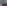
\includegraphics[interpolate=false,width=\linewidth]{content/TemporalerAlg/Bilder/APosteriori/inhomogener_ausschnitt_blocksize.png}
        \caption{inhomogener Pixelblock}
        \label{fig:Inhomogener Pixelblock}
    \end{subfigure}

    \caption{Pixelblöcke bei (in-)homogenen Flächen}\label{fig:Pixelblöcke}
\end{figure}

In einer Gegenüberstellung eines (in-)homogenen Pixelblocks lässt sich die Notwendigkeit der Bildkohärenz erkennen.
In Abbildung \ref{fig:Inhomogener Pixelblock} sind die benachbarten Pixel eine gute Approximation des jeweiligen Pixels, 
wohingegen in Abbildung \ref{fig:homogener Pixelblock} die benachbarten Pixel dies nicht sind.
